\documentclass[10pt,a4paper]{article}
\usepackage[utf8]{inputenc}
\usepackage{amsmath}
\usepackage{amsfonts}
\usepackage{amssymb}
\usepackage{graphicx}

\begin{document}
\title{Projet 4: pre-labo 1}
\date\today
\author{Groupe 7}
\maketitle

\section{Récupération des répliques}
	Afin d'observer les répliques, deux configurations ont été pensée (Figure \ref{conf1} et \ref{conf2}). Dans ces deux situations $d$ est la distance $Tx$ et $Rx$ alors que $x$ est la distance minimale entre $Rx$ (ou $Tx$) et la plaque. Dans ces deux situations, le temps que met l'onde pour passer de $Rx$ à $Tx$ est donné par l'équation \ref{t1}. L'équation \ref{t2} donne le temps du trajet de l'onde réfléchie sur la plaque. $c$ est la vitesse de la lumière. 
	\begin{equation}
	t_1 = \frac{d}{c}
	\label{t1}
	\end{equation}
	
	\begin{equation}
	t_2 = \sqrt{(\frac{d}{2})^2 + x^2} * \frac{1}{c}
	\label{t2}
	\end{equation}
	
	Le première situation sera réalisée pour obtenir un grand $\Delta t$ alors que la seconde pour en obtenir un plus grand. 
	\begin{equation}
	\Delta t = t_2 - t_1 = (\sqrt{(\frac{d}{2})^2 + x^2} - d ) * \frac{1}{c}
	\end{equation}
	
	\begin{figure}[h]
	\centering
	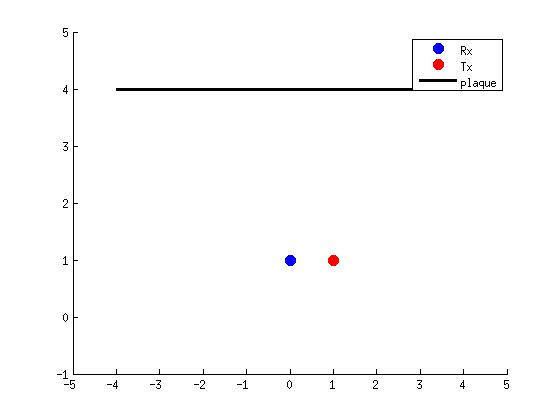
\includegraphics[scale=0.4]{conf1.jpg}
	\caption{Première configuration \label{conf1} }
	\end{figure}		
	
	\begin{figure}[h]
	\centering
	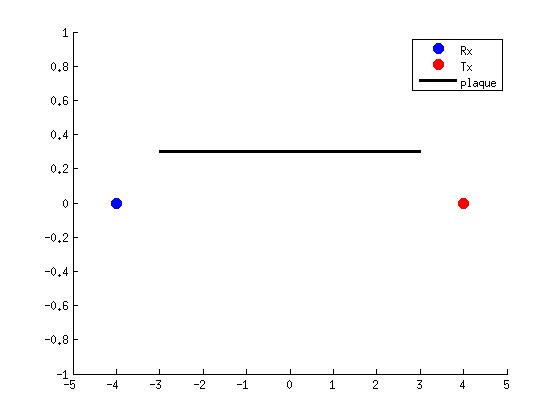
\includegraphics[scale=0.4]{conf2.jpg}
	\caption{Deuxième configuration \label{conf2}}
	\end{figure}		
	

\end{document}
